\documentclass[11pt, oneside]{article}   	% use "amsart" instead of "article" for AMSLaTeX format
\usepackage{hl_short}
\usepackage{geometry}                		% See geom\dagetry.pdf to learn the layout options. There are lots.
\geometry{a4paper}                   		% ... or a4paper or a5paper or ... 
%\geometry{landscape}                		% Activate for for rotated page geometry
%\usepackage[parfill]{parskip}    		% Activate to begin paragraphs with an empty line rather than an indent
\usepackage{graphicx}				% Use pdf, png, jpg, or eps§ with pdflatex; use eps in DVI mode
\usepackage{array}							% TeX will automatically convert eps --> pdf in pdflatex		
\usepackage{amssymb,amsmath}
\usepackage{cite}
\usepackage[final]{fixme}
\usepackage{pdfpages}
\usepackage{tabularx}
\usepackage{fancyheadings}
\usepackage{lastpage}
\usepackage{tikz}
\usetikzlibrary{shapes,arrows}
\usepackage{float}
\usepackage{hyperref}
\usepackage{url}

\newcommand{\comp}[1]{{\sf #1}}

\parskip 6pt % 1pt = 0.351 mm
\parindent 0pt

\pagestyle{fancy}
\lhead{\tiny FP7-ICT 619209 / AMIDST}
\chead{\tiny Page {\thepage} of \pageref{LastPage} \\}
\rhead{\tiny Public}
\renewcommand{\footrulewidth}{0.4pt}
\cfoot{}

\newcommand{\drop}[1]{}

\numberwithin{figure}{section}
\numberwithin{equation}{section}
\numberwithin{table}{section}

\usepackage{pdfpages}

\begin{document}

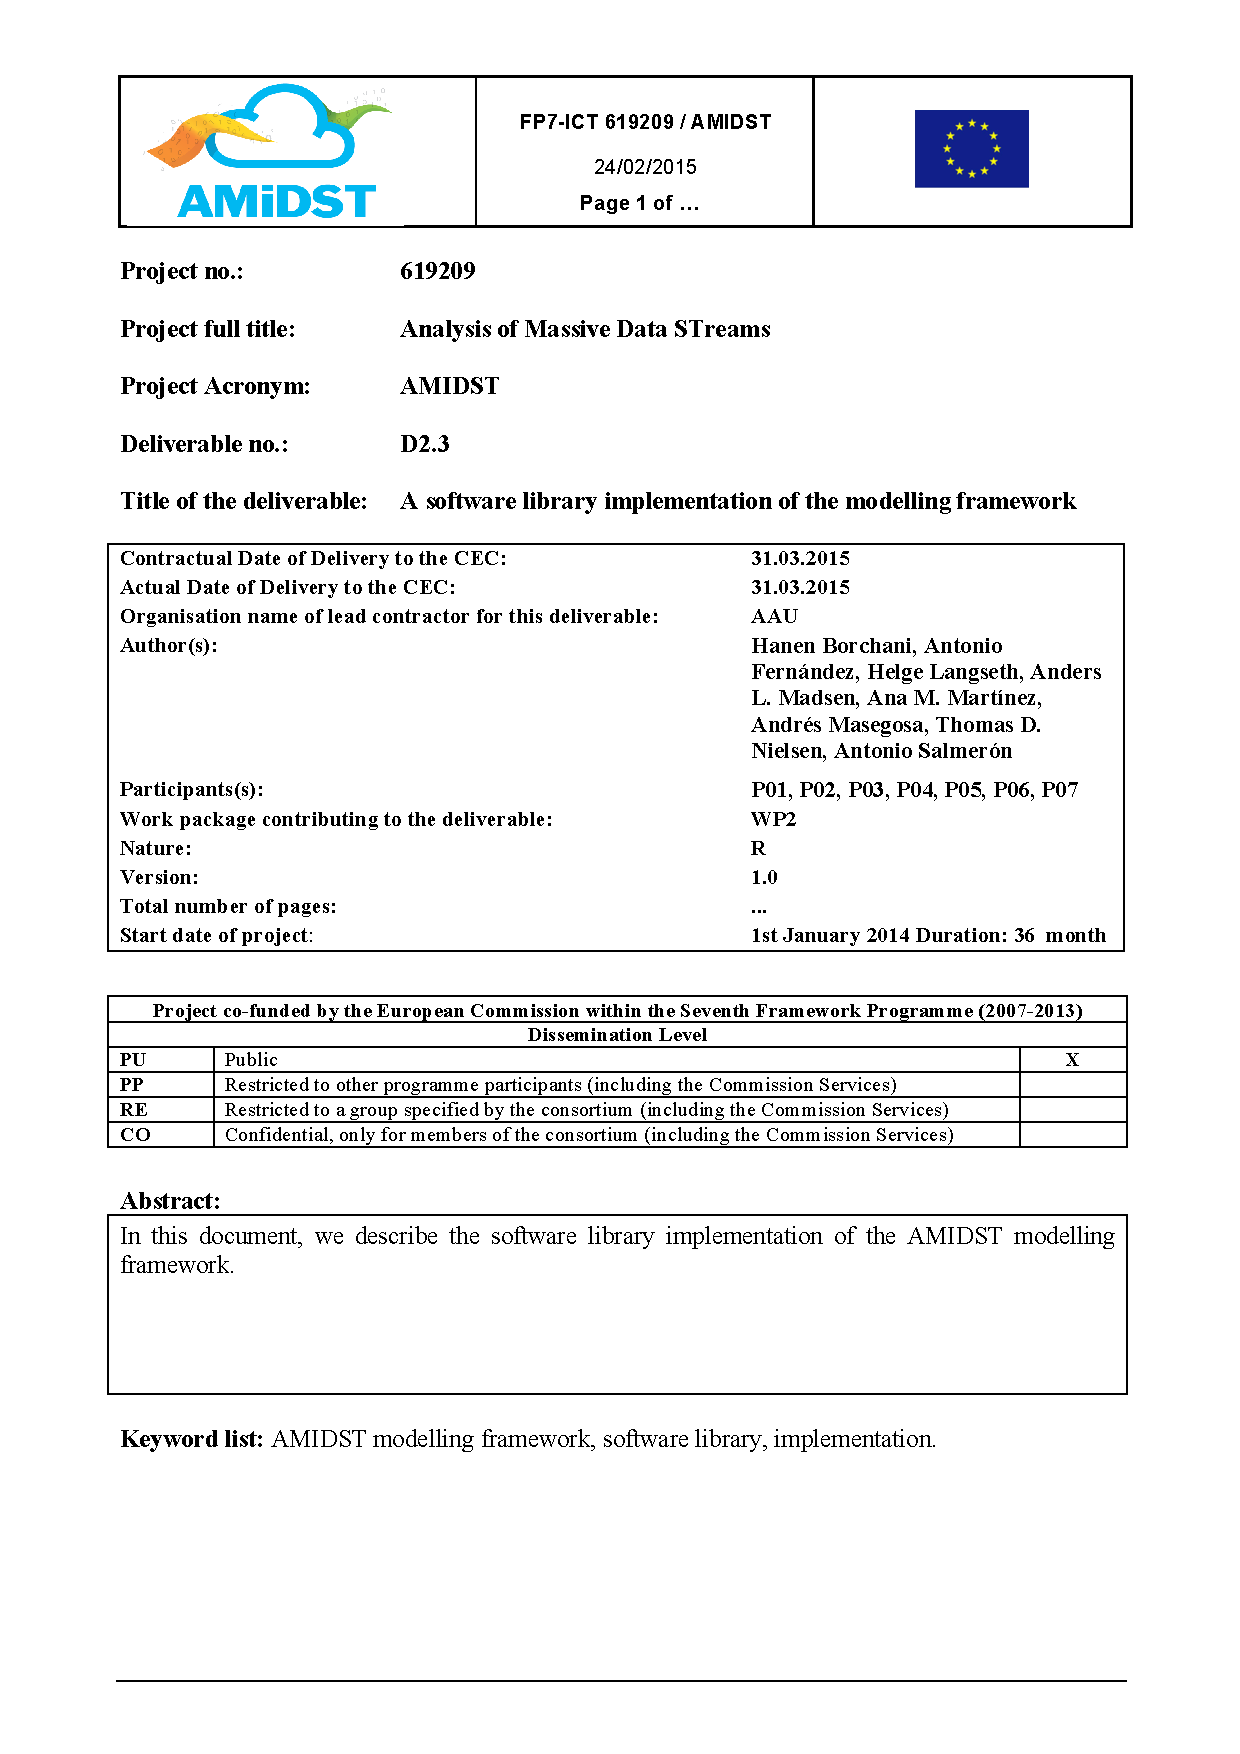
\includepdf[pages={1}]{figures/FrontPage.pdf}

%-------------------------- Table of contents --------------------------
\tableofcontents

\newpage

%-------------------------- Document History --------------------------
\section*{Document history}

\begin{table}[htbp]
  \centering
  \begin{tabularx}{\linewidth}{|p{13mm}| p{18mm}| X | X |} \hline
    {\bf Version} & {\bf Date} & {\bf Author (Unit)} & {\bf Description} \\ \hline
    v0.3 & 10/03/2015~ & All consortium members & The software library implementation for the AMIDST modelling framework discussed and established \\ \hline
    v0.6 & 20/03/2015~ & Hanen Borchani, Antonio Fern\'andez, Ana M. Mart\'inez, Andr\'es Masegosa & Initial version of document finished and reviewed  \\ \hline
    v1.0 & 31/03/2015~ & Hanen Borchani, Antonio Fern\'andez, Helge Langseth, Anders L. Madsen, Ana M. Mart\'inez, Andr\'es Masegosa, Thomas D. Nielsen, Antonio Salmer\'on & Final version of document  \\ \hline
  \end{tabularx}
\end{table}

\newpage

%----------------------------------------------------------------------------
%--------------------------------------------------------------------------------------------------
\section{Executive summary}\label{section:executiveSummary}
%--------------------------------------------------------------------------------------------------

% Consider the diagrams from D4.1
% Extend the functionalities 
% Focus more on inference because it is related to WP3
% Write an introduction to inference (check D3.1, restructure, VMP)
% more details on implemented algorithms
% Description of the implementation with example of use
%----------------------------------------------------------------------------

\newpage

%----------------------------------------------------------------------------
\section{Introduction}

Even though the number of algorithms designed for learning on streaming data is increasing, there is still not a unified and well accepted way for evaluating them.  This is because testing and evaluating algorithms that are designed to work on streaming data are more difficult those designed to work on static data.  There are both statistical and computational reasons for this.  

Static data is data, where each instance can be assumed to be identically and independently distributed i.i.d.  On streaming data, one can often not assume that data instances are i.i.d.  Moreover, the algorithms are often designed to weight measurements that are close to the actual time step higher than measurements that are further back.  On streaming data, we must therefore assume that data are generated from underlying distributions that are time dependent and also that the algorithms themselves are time dependent.  

Computational challenges are related to the fact that the data come from an open-ended data stream, conceptually infinitely long, which imposes practical challenges related to restrictions on cpu-time and memory allocation.  

Various error measures related to stream data has been proposed in the papers of Gama et. al. \cite{Gam09}, \cite{Gam09_2}, \cite{Gam12}.  A loss function is typically related to the penalty of misclassifications on classification problems or residuals in regression models.  The holdout error is basically the average loss on a holdout dataset of fixed size.  The predictive sequential, or \emph{prequential} error is defined as the average loss function up to time step $i$, where $i$ is the current time step.  Moreover, it was also suggested to use a prequental error measure, which involved a forgetting factor such as using a time window or fading factors.  In paper \cite{Gam12}, convergence towards the Bayes error was shown for all these performance measures provided that the learners are consistent and data are i.i.d.  Moreover, it was shown that if data was allowed to drift over time, meaning that samples are only locally i.i.d, then the prequental error measures with forgetting mechanisms were favourable.

\todo{Relate to other work on streaming data as well.}

The applications that are covered in this report have different characteristics than the applications discussed in \cite{Gam12}.  Some problem will be evaluated on a holdout dataset assuming i.i.d and a stationary algorithm.  Other problems can not assume i.i.d on a local scale, but stationarity can be assumed on a larger time scale.  

In this paper we will establish formal procedures for testing and evaluating the developed models and algorithms. This includes specification what metrics are relevant to use to quantify the ability of the AMIDST system, such as relevant formalization of loss functions, maximum response-times, memory limits and output format.  The paper will also include 
considerations about what quantitative improvements AMIDST should obtain over state of the art.

In section \ref{sec:methodology}, AMIDST relevant methodologies for evaluation of both batch and streaming algorithms are identified and discussed.  This section forms the foundation of the subsequent sections, where the exact evaluation routines for each use case provider is given. These sections contains a description of the requirements related to evaluation as described in Delivery 1.2, a short description of the algorithms and the data and finally methods for evaluating predictive and runtime performances.  Section \ref{sec:conclusion} concludes the report.


%\quote{\emph{Task description: In this task we will establish formal procedures for testing and evaluating the
%    developed models and algorithms. This includes specification of maximum response-times, output format,
%    relevant formalization of loss functions, investigations into what metrics are relevant to use to quantify
%    the ability of the AMIDST system, and considerations about what quantitative improvements AMIDST should
%    obtain over state of the art.}}
%
%
%From Helge's slides at the WP 3 kickoff meeting:
%\begin{itemize}
%\item Massive datasets: find relevant techniques, ensure scalability, etc.
%\item Online evaluation of streams: find relevant techniques, ensure scalability, define behavior in changing environment, etc.
%\item Significance of results, e.g., considering changing environment vs. ``reproducability'', distribution for test-statistic, significance levels/sizes of test-sets, etc.
%\end{itemize}

%----------------------------------------------------------------------------

%----------------------------------------------------------------------------
\section{Preliminaries}\label{Section:Preliminaries}

%BN, OOBN, Dynamic BN.
%Preliminaries for the temporal series data analysis: correlograms, partial correlograms. %Preliminaries for the AMIDST models.
%----------------------------------------------------------------------------

%----------------------------------------------------------------------------
%--------------------------------------------------------------------------------------------------
\section{Content of the AMIDST software} \label{sec:Content}
%--------------------------------------------------------------------------------------------------

The AMIDST software is an open source Java project based on Maven automation tool. Maven ensures a description of how the software project is built and its dependencies on other external modules, Java libraries, and plug-ins.  

The AMIDST software consists of:

\begin{itemize}

\item A README file containing a short description of the content of the toolbox, and information on how to compile and run the command line application.

\item The script \texttt{compile.sh} that compiles the whole AMIDST project and create a \texttt{.jar} file in the ./target folder.

\item The script \texttt{run.sh} that should be used to run some classes. For instance, \texttt{./run.sh} \texttt{eu.amidst.examples.DynamicNaiveBayesClassifierDemo} runs a demo for learning a dynamic naive Bayes classifier.

\item The source code organised in packages, as shown in Figure \ref{Figure:SoftwareContent}, and consisting of the implementation of the data structures, the database functionalities, the AMIDST models, and the different considered algorithms for learning and inference. 

\end{itemize}


\begin{figure}[ht!]
\begin{center}
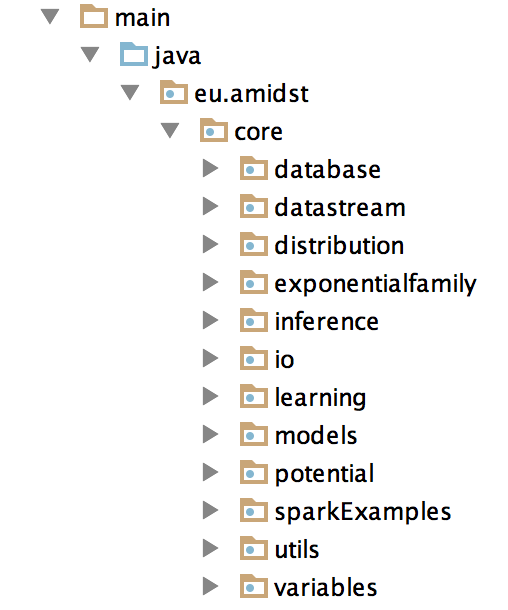
\includegraphics[scale=0.75]{./figures/SoftwareContent}
\caption{\label{Figure:SoftwareContent}Content of the AMIDST software.}
\end{center}
\end{figure}
%----------------------------------------------------------------------------

%----------------------------------------------------------------------------
%------------------------------------------------------------------------------------------------------------
\section{Data structures} \label{sec:DataStructures}
%------------------------------------------------------------------------------------------------------------

An overview of the different data structures of the AMIDST toolbox is illustrated in Figure \ref{Figure:ToolboxDataStructures}. These data structures basically define the main components that are used afterwards for implementing the AMIDST learning and inference algorithms. In what follows, we briefly define each component showing how it can be used through providing some code excerpts. 

\begin{figure}[ht!]
\begin{center}
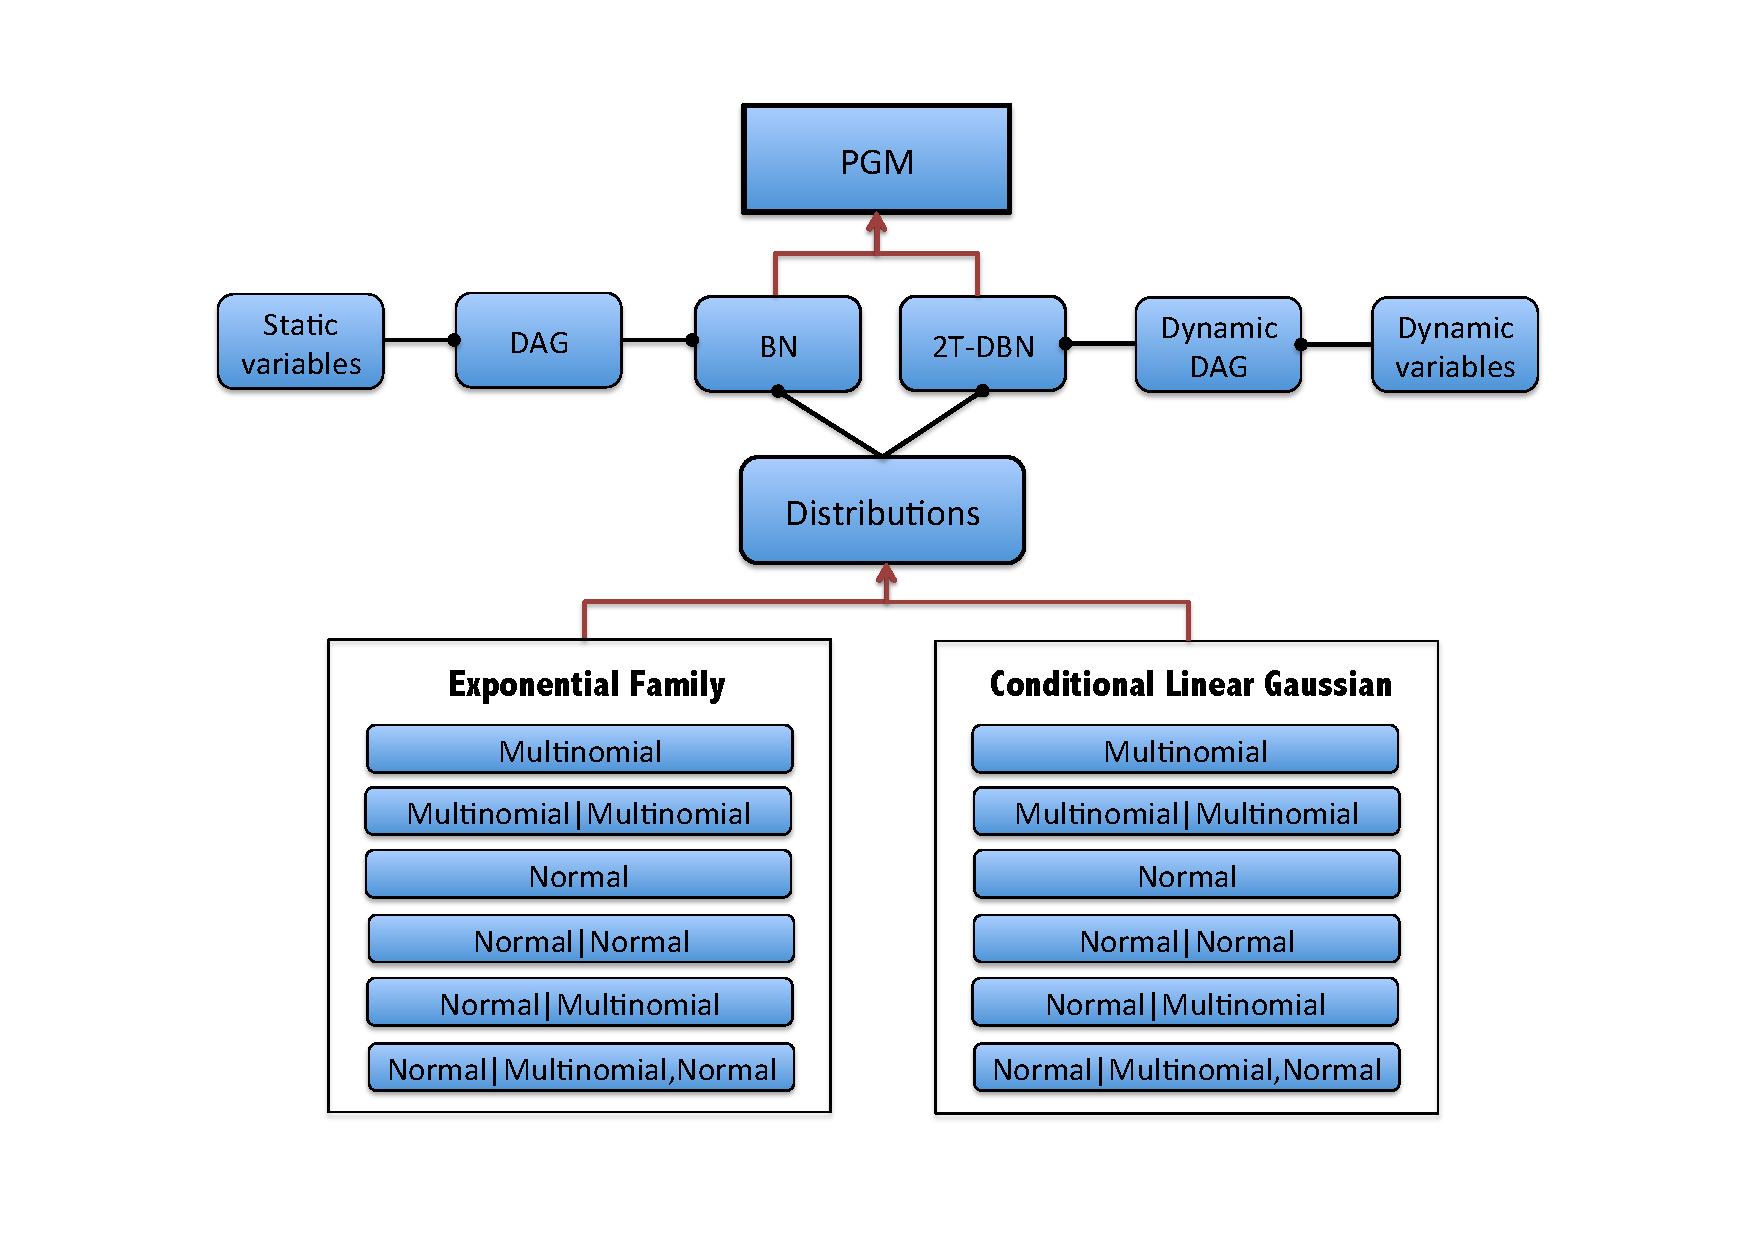
\includegraphics[width=\linewidth]{./figures/DataStructure}
\caption{\label{Figure:ToolboxDataStructures} Illustration of AMIDST toolbox data structure components. Nomenclature: The boxes in the
      figure represent software components (sets, possibly singletons, of classes), a rounded-arc going from $X$ to $Y$ indicates that $Y$ 'uses/references' $X$, and an arc with an arrow from $X$ to $Y$ implies inheritance.}
\end{center}
\end{figure}

%------------------------------------------------------------------------------------------------------------
\subsection{Probabilistic graphical model (\comp{PGM})}
%------------------------------------------------------------------------------------------------------------

 A probabilistic graphical model is a framework consisting of two parts: a qualitative component in the form of a graphical model encoding conditional independence assertions about the domain being modelled as well as a quantitative component consisting of a collection of local probability distributions adhering to the independence properties specified in the graph- ical model. Collectively, the two components provide a compact representation of the joint probability distribution over the domain being modelled.
 
In the AMIDST toolbox, we currently focus on two specific instantiations of PGMs, namely, a static Bayesian network (\comp{BN} component) and a two time-slice dynamic Bayesian network (\comp{2T-DBN}). 
 

%------------------------------------------------------------------------------------------------------------
\subsection{Static variables}
%------------------------------------------------------------------------------------------------------------

Static variables consist of a list of objects of type \texttt{Variable} that are used later to build a static Bayesian network. Each static variable is characterized by its name, ID, the state space type, the distribution type (i.e., multinomial or normal), as well as if it is observed or not. 

Note that observed static variables are initialised using the list of attributes (that are already parsed from the dataset or specified by the user), then hidden static variables are afterwards specified by the user.

\begin{table}[H]
\begin{tabular}{l} \\ \hline

        \texttt{StaticVariables variables = new StaticVariables(data.getAttributes());}\\

        \texttt{Variable A = variables.getVariableByName("A");}\\
        \texttt{Variable B = variables.getVariableByName("B");}\\
        \texttt{Variable C = variables.getVariableByName("C");}\\\\

        \texttt{VariableBuilder variableBuilder = new VariableBuilder();}\\
        \texttt{variableBuilder.setName("HiddenVar");}\\
        \texttt{variableBuilder.setObservable(false);}\\
        \texttt{variableBuilder.setStateSpace(new }\\  \texttt{~~~~~~MultinomialStateSpace(Arrays.asList("TRUE","FALSE")));}\\
        \texttt{variableBuilder.setDistributionType(DistType.MULTINOMIAL);}\\
        \texttt{Variable hidden = variables.addHiddenVariable(variableBuilder);}\\ \hline 

\end{tabular}
\end{table}


%------------------------------------------------------------------------------------------------------------
\subsection{Directed acyclic graph (\comp{DAG})}
%------------------------------------------------------------------------------------------------------------

A directed acyclic graph (\comp{DAG}) defines the Bayesian network graphical structure over a list of \comp{Static variables}, such that he dependence relationships between the variables are established through the definition of the parent set for each variable. 

\begin{table}[H]
\begin{tabular}{l} \\ \hline

        \texttt{WekaDataFileReader reader = new}\\
         \texttt{~~~~~~WekaDataFileReader("data/dataWeka/contact-lenses.arff");}\\

        \texttt{StaticVariables variables = new StaticVariables(reader.getAttributes());}\\
        \texttt{DAG dag = new DAG(variables);}\\\\

        \texttt{StaticVariables variables = dag.getStaticVariables();}\\
        \texttt{Variable A = variables.getVariableById(0);}\\
        \texttt{Variable B = variables.getVariableById(1);}\\
        \texttt{Variable C = variables.getVariableById(2);}\\
        \texttt{Variable D = variables.getVariableById(3);}\\ \\ 

        \texttt{dag.getParentSet(B).addParent(A);}\\
        \texttt{dag.getParentSet(C).addParent(A);}\\
        \texttt{dag.getParentSet(D).addParent(B);}\\
        \texttt{dag.getParentSet(D).addParent(C);}\\ \hline 

\end{tabular}
\end{table}


%------------------------------------------------------------------------------------------------------------
\subsection{Bayesian network (\comp{BN})}
%------------------------------------------------------------------------------------------------------------

A static Bayesian network consists of two components: a graphical structure (defined by the \comp{DAG} component) and conditional probability distributions of each variable given the set of its parents (defined by the \comp{Distributions} component).

The distribution of each variable in the Bayesian network is initialised and specified according to its type and the type of its potential parent set. After this step, the set of parents of each variable becomes unmodifiable.

This is brief code fragment showing the definition of a Bayesian network using the previously created \comp{dag}. It automatically looks at the distribution type of each variable and their parents to initialise the Distributions objects that are stored inside (i.e., Multinomial, Normal, CLG, etc). The parameters defining these distributions are correspondingly initialised.

\begin{table}[H]
\begin{tabular}{l} \hline\\ 
        \texttt{BayesianNetwork bn = BayesianNetwork.newBayesianNetwork(dag);}\\ \\ \hline 
\end{tabular}
\end{table}      


%------------------------------------------------------------------------------------------------------------
\subsection{Dynamic variables}
%------------------------------------------------------------------------------------------------------------

Dynamic variables consist of a list of objects named allVariables and temporalClones of type \texttt{Variable}, that are used to build dynamic Bayesian networks. Each dynamic variable is characterized by its name, ID, the state space type, the distribution type (i.e., multinomial or normal), and if it is observed or not. In order to represent the variables in a previous time step (needed when defining the dynamic DAG), we use the concept of \textit{temporal clone} variables, which are copies of the real main variables but refer to the previous time step. For instance, $X_{t-1}$ is codified as the \textit{temporal clone} of variable $X_t$. Hence, in our data structures, the time index $t$ is not explicitly represented for a dynamic variable, but implicitly considered with the use of \textit{temporal clones}.

The list of observable dynamic variables and their temporal clones is initialised using the list of Attributes (that are already parsed from the dataset or specified by the user), then hidden variables and their temporal clones can be also added by the user.

\begin{table}[H]
\begin{tabular}{l} \\\hline

        \texttt{DynamicVariables dynamicVariables = new DynamicVariables();}\\

        \texttt{Variable observedROP = dynamicVariables.addObservedDynamicVariable(attROP);}\\
        \texttt{Variable observedTRQ = dynamicVariables.addObservedDynamicVariable(attTRQ);}\\
        \texttt{Variable realTRQ = dynamicVariables.addRealDynamicVariable(observedTRQ);}\\

        \texttt{VariableBuilder variableBuilder = new VariableBuilder();}\\
        \texttt{variableBuilder.setName("HiddenVar");}\\
        \texttt{variableBuilder.setObservable(false);}\\
        \texttt{variableBuilder.setStateSpace(new RealStateSpace()); }\\
        \texttt{variableBuilder.setDistributionType(DistType.GAUSSIAN);}\\
        \texttt{Variable hidden = dynamicVariables.addHiddenDynamicVariable(variableBuilder);}\\ \hline 

\end{tabular}
\end{table}

%------------------------------------------------------------------------------------------------------------
\subsection{Dynamic directed acyclic graph (\comp{Dynamic DAG})}
%------------------------------------------------------------------------------------------------------------

A dynamic directed acyclic graph (\comp{Dynamic DAG}) defined over a list of \comp{dynamic variables}. This component specifies the graph structure of a \comp{2T-DBN}, i.e., the parent set for each dynamic variable at both time $0$ and at time $t > 0$. 

\begin{table}[H]
\begin{tabular}{l} \\ \hline
        \texttt{DynamicDAG dynamicDAG = new DynamicDAG(dynamicVariables);}\\\\
        
        \texttt{dynamicDAG.getParentSetTimeT(observedTRQ).addParent(observedWOB);}\\
        \texttt{dynamicDAG.getParentSetTimeT(observedTRQ).addParent(observedRPMB);}\\
        \texttt{dynamicDAG.getParentSetTimeT(observedTRQ).addParent(observedMFI);}\\
        \texttt{dynamicDAG.getParentSetTimeT(observedTRQ).addParent(realTRQ);}\\
        \texttt{dynamicDAG.getParentSetTimeT(observedTRQ).addParent(hidden);}\\
        \texttt{dynamicDAG.getParentSetTimeT(observedTRQ).addParent(mixture);}\\  \hline 
\end{tabular}
\end{table}

%------------------------------------------------------------------------------------------------------------
\subsection{Two time-slice dynamic Bayesian network (\comp{2T-DBN})}
%------------------------------------------------------------------------------------------------------------

Similarly to a BN, a 2T-DBN (see Deliverable D2.1, Section 3.4 \cite{Deliverable2.1}) is defined using two main components: a graphical structure (defined by the \comp{Dynamic DAG} component) and conditional probability distributions of each dynamic variable given the set of its parents (defined by the \comp{Distributions} component). The distributions of each dynamic variable at both time 0 and time T are initialised and specified according to the variable type and the type of its potential parent set. After this step, the set of parents of each dynamic variable becomes unmodifiable.

This is brief code fragment showing the definition of a dynamic Bayesian network using the previously created \texttt{dynamicDAG}. It automatically looks at the distribution type of each variable and their parents to initialise the Distributions objects that are stored inside (i.e., Multinomial, Normal, CLG, etc). The parameters defining these distributions are correspondingly initialised.

\begin{table}[H]
\begin{tabular}{l} \\ \hline

        \texttt{DynamicBayesianNetwork dynamicBayesianNetwork = }\\ \texttt{ DynamicBayesianNetwork.newDynamicBayesianNetwork(dynamicDAG);}\\\\ \hline 
\end{tabular}
\end{table}


%------------------------------------------------------------------------------------------------------------
\subsection{Distributions}
%------------------------------------------------------------------------------------------------------------

The \comp{Distributions} component consists of the set of conditional probability distributions considered in the AMIDST toolbox, including variables with both multinomial and normal distributions. 

Note here that, in spite of the distinction between \comp{BN} and \comp{2T-BN}, the distributions over both models could be defined in the same way, and thereby the parameter learning and inference algorithms could be also applied equally for both models. In particular, the \comp{Distributions} component includes the set of conditional probability distributions considered in the AMIDST toolbox (the so-called \comp{Conditional Linear Gaussian} distributions, as detailed in Deliverable 2.1 \cite{Deliverable2.1}). More precisely, both variables with multinomial and normal distributions are modeled, and the distribution of each variable, in either a \comp{BN} or \comp{2T-BN}, is initialized and specified according to its distribution type and the distribution types of its potential parents. This consequently gives rise to the following different implemented probability distributions:

\begin{itemize}
  \item \comp{Multinomial}: a multinomial variable with no parents.
  \item \comp{Multinomial$|$Multinomial}: a multinomial variable with multinomial parents.
  \item \comp{Normal}: a normal variable with no parents.
  \item \comp{Normal$|$Normal}: a normal variable with normal parents.
  \item \comp{Normal$|$Multinomial}: a normal variable with multinomial parents.
  \item \comp{Normal$|$Multinomial,Normal}: a normal variable with a mixture of multinomial and normal parents.
\end{itemize}

The case of a multinomial variable having normal parents is not considered yet in this initial prototype. It is planned to be included in future versions, although strongly restricted in inference and learning algorithms due to the methodological and computational issues previously commented in Deliverable D2.1 \cite{Deliverable2.1}. 

We also provide an implementation of all the above distributions in the so-called \comp{Exponential Family} form, which ensures an alternative representation of the standard distributions based on vectors of natural and moment parameters.

The following brief code fragment shows the definition of the distribution for a variable \texttt{var} given the set of its parents:

\begin{table}[H]
\begin{tabular}{l} \hline

        \texttt{ParentSet parentSet = this.getDAG().getParentSet(var);}\\
        \texttt{int varID = var.getVarID();}\\

        \texttt{this.distributions[varID]= }\\
         \texttt{~~~~~DistributionBuilder.newDistribution(var, parentSet.getParents());}\\
        \texttt{parentSet.blockParents();}\\ \hline 

\end{tabular}
\end{table}

%----------------------------------------------------------------------------

%----------------------------------------------------------------------------
%------------------------------------------------------------------------------------------------------------
\section{Database management} \label{sec:DataBases}
%------------------------------------------------------------------------------------------------------------

This section covers the description of databases that will be used later by AMIDST learning and inference algorithms implemented in the toolbox.  Figure~\ref{fig:DataBase} shows a high-level overview of the key components of the AMIDST toolbox. It illustrates mainly the different database functionalities and how they are connected to the core component \comp{PGM} through both the \comp{Learning Engine} and \comp{Inference Engine} components. In what follows, we describe each of the database functionalities, along with a code excerpt containing a brief example, then we introduce briefly the \comp{Learning Engine} and \comp{Inference Engine} that will be presented in more details in Deliverable 3.2.

\vspace{-0.4in}
  \begin{figure}[ht!]
    \centering
    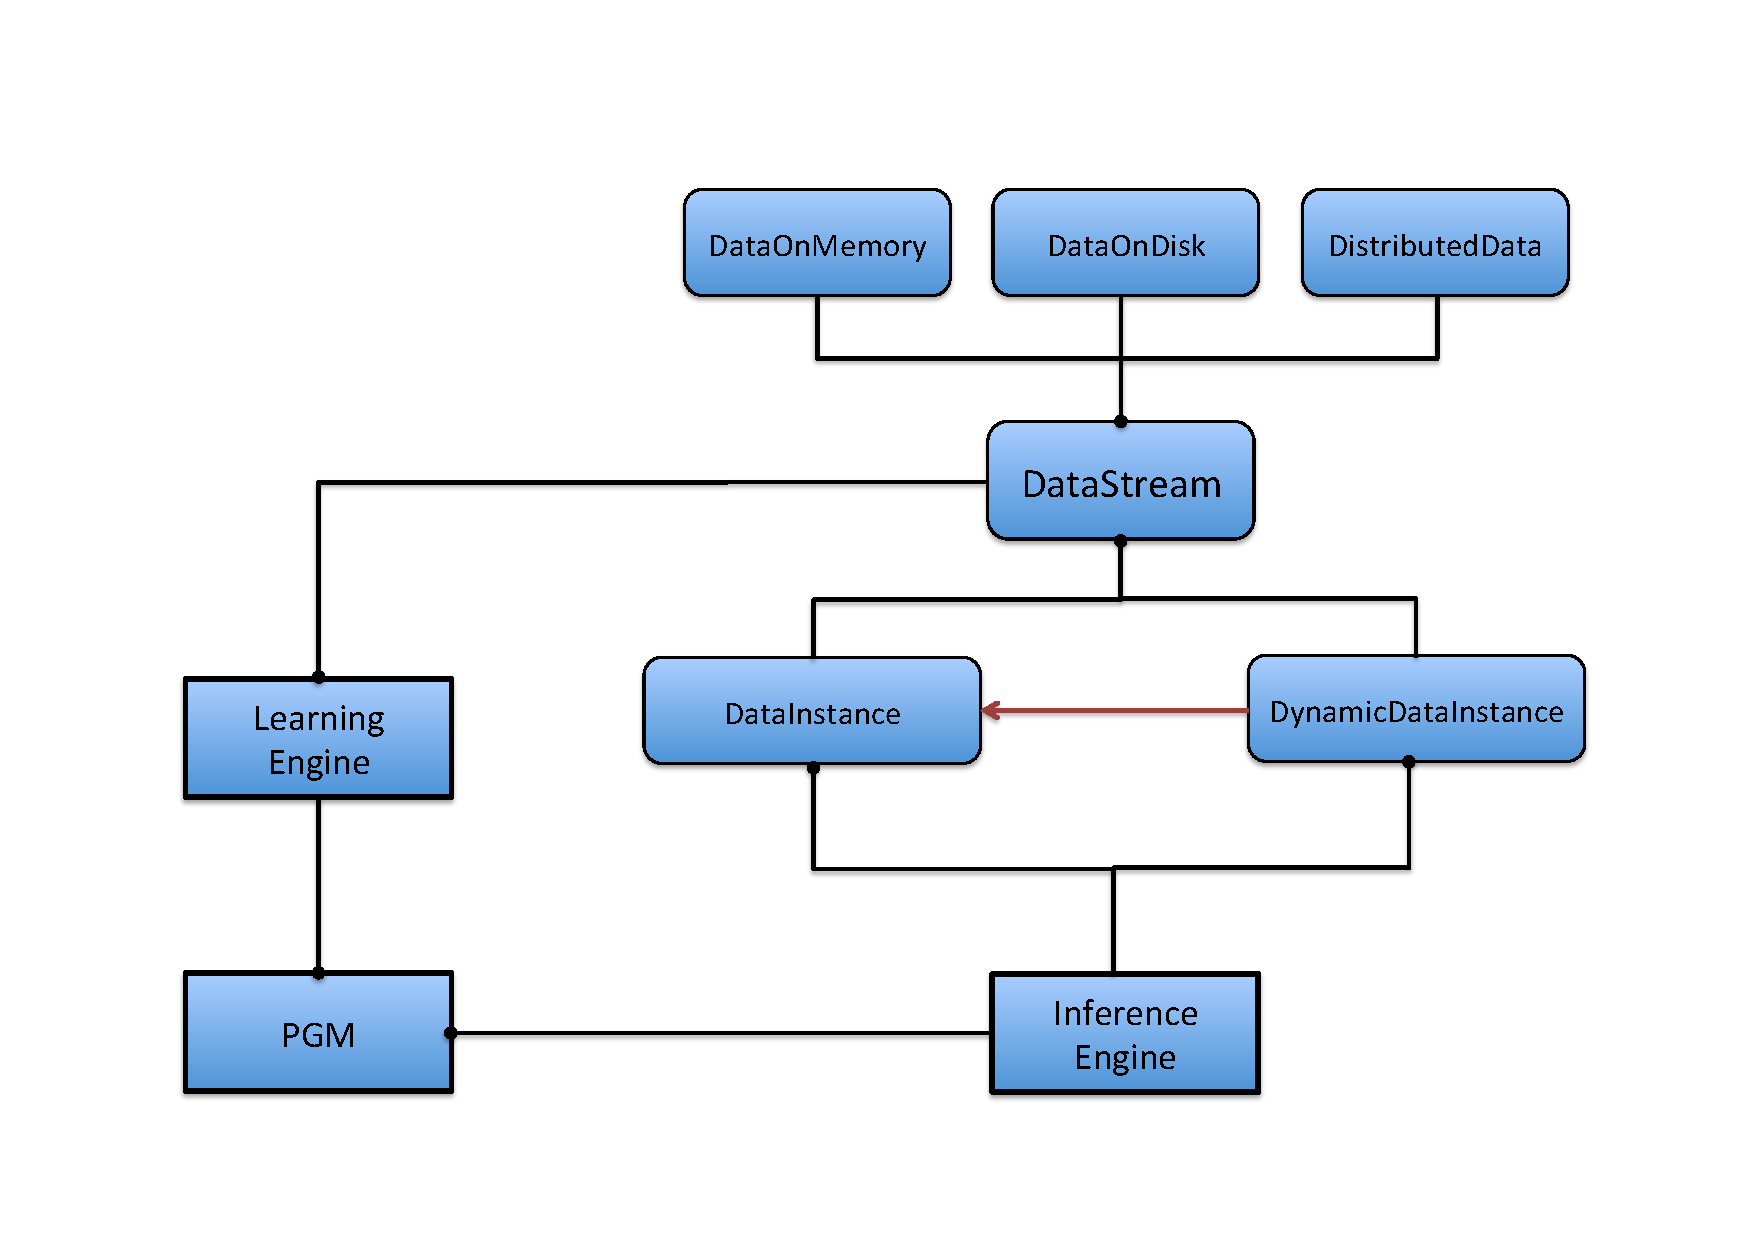
\includegraphics[width=\linewidth]{./figures/DataBase}
    \vspace{-0.8in}
    \caption{Illustration of the main database management functionalities and their connection with PGM, learning engine, and inference engine components. }
    \label{fig:DataBase}
  \end{figure}
 
%------------------------------------------------------------------------------------------------------------
\subsection{DataStream}
%------------------------------------------------------------------------------------------------------------   

In the AMIDST framework, we consider a \comp{DataStream} as a data source, i.e., a streaming data where records arrive at high frequency with no storage of historical data in memory. \comp{DataStream} is connected to either \comp{DataInstance} and \comp{DynamicDataInstance} components. 

The employed design is intended to support future users and developers of the AMIDST toolbox in the potential design and implementation of other database specifications; the only restriction being that new database components should implement the interface defined by the \comp{DataStream} component. 

%------------------------------------------------------------------------------------------------------------
\subsection{DataInstance}
%------------------------------------------------------------------------------------------------------------  
  
The \comp{DataInstance} component consists of a single class that represents a particular evidence configuration, such as the observed values of a collection of variables in a particular data row. 


\vspace{-0.1in}
\begin{table}[H]
\begin{tabular}{l} \\ \hline
                \texttt{DataStream<DataInstance> data = }\\
                 \texttt{~~~~~~~~~~DataStreamLoader.loadFromFile("datasets/staticData.arff");}\\\hline 
\end{tabular}
\end{table}

%------------------------------------------------------------------------------------------------------------
\subsection{DynamicDataInstance}
%------------------------------------------------------------------------------------------------------------  

The \comp{DynamicDataInstance} component consists of two data rows, such that the first refers to the past while the second refers to the present. In addition to the attributes present in each data row, \comp{DynamicDataInstance} could be characterised also with a TimeID and a SequenceID stored as additional attributes in the considered dynamic data.

\vspace{-0.1in}
\begin{table}[H]
\begin{tabular}{l} \\ \hline
        \texttt{DataStream<DynamicDataInstance> data = }\\
        \texttt{~~~~ DynamicDataStreamLoader.loadFromFile("datasets/dynamicData.arff");}\\\hline 
\end{tabular}
\end{table}


%------------------------------------------------------------------------------------------------------------
\subsection{Learning Engine}
%------------------------------------------------------------------------------------------------------------  

The \comp{Learning Engine} component consists of the implementations of the different learning algorithms for static and dynamic BNs, ensuring both structural and parameter learning. For structural learning, the AMIDST toolbox currently supports standard PC and parallel TAN algorithms by interfacing to the Hugin API (cf.\ Task 4.1). For parameter learning, a fully Bayesian approach is pursued in the AMIDST framework (cf.\ Task 4.2 and Task 4.4), which means that parameter learning reduces to the task of inference for which two approaches will be considered:, namely, variational message passing and expectation propagation. 

More implementation details about these algorithms will be provided in Deliverable 3.2. Note also that the design of the \comp{Learning Engine} is flexible in the sense that it easily accommodates potential future learning-based extensions, such as Bayesian learning based on importance sampling or maximum likelihood learning using the expectation maximization algorithm (see Section 3 in Deliverable 4.1 \cite{Deliverable4.1}). 
 
%------------------------------------------------------------------------------------------------------------
\subsection{Inference Engine}
%------------------------------------------------------------------------------------------------------------  

The \comp{Inference Engine} component consists of the implementations of both variational message passing and expectation propagation algorithms 
for probabilistic graphical models with conjugate-exponential distribution families (see Section 3, Deliverable 4.1 \cite{Deliverable4.1}). 

The different functionalities of the \comp{Inference Engine} component are ensured in AMIDST toolbox through tailored exponential family implementations of the standard distributions that are part of the AMIDST framework (such as the conditional linear Gaussian distributions). More details about this component will be provided in Deliverable 3.2.  
%----------------------------------------------------------------------------

%----------------------------------------------------------------------------
%------------------------------------------------------------------------------------------------------------
\section{HUGIN AMIDST API} \label{sec:HuginLink}
%------------------------------------------------------------------------------------------------------------

The \comp{Hugin link} component consists of the functionalities implemented to link the AMIDST toolbox with the HUGIN software. This connection is primarily ensured by converting HUGIN models into AMIDST models, and vice versa. 

This component is extremely useful as it allows us to test and assess some of the implemented AMIDST functionalities within a well-established platform as HUGIN. For instance, a new inference algorithm implemented in AMIDST could be compared with some state-of-the-art algorithms included in HUGIN. In addition, the connection with HUGIN efficiently extends AMIDST toolbox by providing some extra functionalities, such as the use of parallel TAN for BN structural learning. 

%------------------------------------------------------------------------------------------------------------
\subsection{Converters from AMIDST to HUGIN format} \label{ConverterFromAmidstToHugin}
%------------------------------------------------------------------------------------------------------------

This functionality addresses the conversion of a \comp{BN} or a \comp{DBN} from AMIDST to HUGIN. This conversion is done at ``object-level'', which is far more efficient that if it would be done by converting the models to data files and, then, parsing them. 

The following brief code fragment shows how to convert a \comp{BN} and a \comp{DBN} from AMIDST to HUGIN format, then store them in files. The files could be then accessed and opened using HUGIN software to visually check the created networks with the AMIDST toolbox. 


\begin{table}[H]
\begin{tabular}{l} \hline

\%For a \comp{BN}:\\ 
\texttt{BayesianNetwork amidstBN = BayesianNetwork.newBayesianNetwork(dag);}\\
\texttt{Domain huginBN = BNConverterToHugin.convertToHugin(amidstBN);;}\\
\texttt{huginBN.saveAsNet("networks/huginNetworkFromAMIDST.net");}\\\\ 

\%For a \comp{DBN}:\\ 
        \texttt{DynamicBayesianNetwork amidstDBN =}\\ \texttt{~~~~~DynamicBayesianNetwork.newDynamicBayesianNetwork(dynamicDAG);}\\
        \texttt{Class huginDBN = DBNConverterToHugin.convertToHugin(amidstDBN);}\\
        \texttt{huginDBN.setName("huginDBNFromAMIDST");}\\
        \texttt{huginDBN.saveAsNet("networks/huginDBNFromAMIDST.oobn");}\\ \hline

\end{tabular}
\end{table} 

%------------------------------------------------------------------------------------------------------------
\subsection{Converters from HUGIN to AMIDST format} \label{ConverterFromHuginToAmidst}
%------------------------------------------------------------------------------------------------------------

This functionality addresses the conversion of a \comp{BN} or a \comp{DBN} from HUGIN to AMIDST. As before, this conversion is also done at ``object-level''.

The following brief code fragment shows how to convert a \comp{BN} and a \comp{DBN} from HUGIN to AMIDST format, then store them in files. The files could be then accessed and used in AMIDST toolbox. 


\begin{table}[H]
\begin{tabular}{l} \hline

\%For a \comp{BN}:\\ 

        \texttt{ParseListener parseListener = new DefaultClassParseListener();}\\
        \texttt{Domain huginBN = new Domain ("networks/asia.net", parseListener);}\\
        \texttt{BayesianNetwork amidstBN = BNConverterToAMIDST.convertToAmidst(huginBN);}\\
        \texttt{BayesianNetworkWriter.saveToFile(amidstBN, "networks/asia.bn");}\\\\

\%For a \comp{DBN}:\\ 
        \texttt{DefaultClassParseListener parseListener = new DefaultClassParseListener();}\\
        \texttt{ClassCollection cc = new ClassCollection();}\\
        \texttt{String file = new String("networks/CajamarDBN.oobn");}\\
        \texttt{cc.parseClasses (file, parseListener);}\\
        \texttt{String[] aux = file.split("/");}\\
        \texttt{String fileName = aux[aux.length-1];}\\
        \texttt{String modelName = fileName.substring(0,fileName.length()-5);}\\
        \texttt{Class HuginDBN = cc.getClassByName(modelName);}\\
        \texttt{DynamicBayesianNetwork amidstDBN = DBNConverterToAmidst.convertToAmidst(HuginDBN);}\\
        \texttt{DynamicBayesianNetworkWriter.saveToFile(amidstDBN, "networks/CajamarDBN.bn");}\\ \hline
        
\end{tabular}
\end{table} 
%----------------------------------------------------------------------------

%----------------------------------------------------------------------------
\section{Conclusion, observations and reflections} \fixme{For a
  possible publication, we could report on our (including the use case providers') experiences with the process, but
  since we are not yet finish with the RE process there is not that much to report \ldots }
\label{sec:conclusion}

This document describes the requirement engineering process pursued in AMIDST. The general process is  adapted and based
on previously described approaches to requirements engineering, but tailored to the specific needs and characteristics of the AMIDST
project. In particular, the idiosyncratic aspects of the AMIDST project that combined distinguishes it from other software
projects at the requirements engineering level, include (i) a pre-defined project scope, (ii) many different
stakeholders, and (iii) the development of a sufficiently general software framework that can be instantiated for
use case providers representing different industries.  Central to the requirements engineering approach is the use case
concept that forms the basis for the requirements specification. The actual specification is document in a generic
formal template that allows for the elicited requirements to be compared and prioritized across domains. 

The division of work realized in the AMIDST project was partly successful due to the natural coupling (geographical and
affinity based) between the industrial partners and the academic partners. This type of work division may not be
achievable in projects with a larger number of partners or where the partners are not geographical co-located. On the
other hand, it should also be emphasized that this division of work is \emph{not} as such prescribed by the proposed
requirements engineering process. 

%----------------------------------------------------------------------------

\bibliographystyle{splncs}

\bibliography{biblio}

\end{document}  